\documentclass[en,oneside,onehalfspacing,msc]{risethesis}

\usepackage[english]{babel}
\usepackage[utf8]{inputenc}
\usepackage[linesnumbered,vlined,ruled,boxed,commentsnumbered]{algorithm2e}
\usepackage{algpseudocode}
\usepackage{bm} % Allows bold greek letters for representing vectors

% math equations
\usepackage{amsmath,amssymb,amsfonts}
\usepackage{commath}
\usepackage{float}

\usepackage[flushleft]{threeparttable}

\usepackage{colortbl}
\usepackage{color}
\usepackage[table]{xcolor}
\usepackage{microtype}
\usepackage{bibentry}
\usepackage{subfig}
\usepackage{multirow}
\usepackage{rotating}
\usepackage{booktabs}
\usepackage{pdfpages}
\usepackage{lipsum}
\usepackage{scalefnt}

\let\counterwithout\relax
\let\counterwithin\relax
\usepackage{chngcntr}

\usepackage[tocflat,toctextentriesindented]{tocstyle}
\deactivatetocstyle[lof]
\deactivatetocstyle[lot]
\deactivatetocstyle[loa]

\usetocstyle{allwithdot}
\settocfeature[toc][0]{entryhook}{\bfseries\uppercase}
\settocfeature[toc][1]{entryhook}{\uppercase}
\settocfeature[toc][2]{entryhook}{\bfseries}
\settocfeature[toc][3]{entryhook}{\itshape}

\settocfeature{spaceafternumber}{3em}
\makeatletter
\renewcommand*\l@figure{\@dottedtocline{1}{1.5em}{5.9em}}
\renewcommand*\l@table{\@dottedtocline{1}{1.5em}{5em}}
\makeatother

\usepackage{titlesec}
\titleformat{\section}{\normalfont\large}{\thesection}{1em}{\MakeUppercase}
\titleformat{\subsection}{\normalfont\large}{\bfseries\thesubsection}{1em}{\bfseries}
\titleformat{\subsubsection}{\normalfont\large}{\itshape\thesubsubsection}{1em}{\itshape}

\newcommand{\fref}[1]{Figure \ref{#1}}
\newcommand{\tref}[1]{Table \ref{#1}}
\newcommand{\sref}[1]{Section \ref{#1}}
\newcommand{\eref}[1]{Equation \ref{#1}}
\newcommand{\aref}[1]{Algorithm \ref{#1}}
\newcommand{\chref}[1]{Chapter \ref{#1}}

% \captionsetup[table]{position=top,justification=centering,width=.85\textwidth,font=small, labelsep=newline}
%\captionsetup[lstlisting]{position=top,justification=centering,width=.85\textwidth,labelfont=bf,font=small}
%\captionsetup[figure]{position=bottom,justification=centering,width=.85\textwidth,labelfont=bf,font=small}

% -----------------------------------------------------------
% settings for the list of acronyms
% begin
% -----------------------------------------------------------
% \usepackage[noredefwarn,acronym]{glossaries} %GLOSSÁRIO

\newcolumntype{L}[1]{>{\raggedright\let\newline\\\arraybackslash\hspace{0pt}}m{#1}}
\newcolumntype{C}[1]{>{\centering\let\newline\\\arraybackslash\hspace{0pt}}m{#1}}
\newcolumntype{R}[1]{>{\raggedleft\let\newline\\\arraybackslash\hspace{0pt}}m{#1}}

\newglossarystyle{modsuper}{%
  \setglossarystyle{super}%
  \renewcommand{\glsgroupskip}{}

  % put the glossary in a longtable environment:
 \renewenvironment{theglossary}%
  {
    \begin{longtable}
        {L{0.3\textwidth}L{0.7\textwidth}}}%
    {\end{longtable}
    \addtocounter{table}{-1}
  }
}

% -----------------------------------------------------------
% settings for the list of acronyms
% end
% -----------------------------------------------------------

%% Change the following pdf author attribute name to your name.
\usepackage[linkcolor=black,
            citecolor=blue,
            urlcolor=black,
            colorlinks,
            pdfpagelabels,
            pdftitle={M.Sc. Dissertation - Author's Name},
            pdfauthor={Author's Name}]{hyperref}

\address{Recife}

\universitypt{Universidade Federal de Pernambuco}
\universityen{Federal University of Pernambuco}

\departmentpt{Centro de Informática}
\departmenten{Center of Informatics}

\programpt{Pós-graduação em Ciência da Computação}
\programen{Graduate in Computer Science}

\majorfieldpt{Ciência da Computação}
\majorfielden{Computer Science}

\concentrationareapt{Inteligência Computational}
\concentrationareaen{Computational Intelligence}

\title{Title}

\date{2019}

\author{Author's name}
\adviser{Professor's name}

% Macros (defines your own macros here, if needed)
\def\x{\checkmark}

\setlength{\headheight}{16pt} %Solucao para o Erro:Package Fancyhdr Warning: \headheight is too small (12.0pt)

% ----------------------------------------------------------
% import list of acronyms and symbols
% ----------------------------------------------------------
\newacronym{som}{SOM}{Self-Organizing Map}
\newacronym{svhn}{SVHN}{Street View House Numbers}
\newacronym{cifar10}{CIFAR10}{Canadian Institute For Advanced Research}

\newglossaryentry{updatestep}{
  name = $\Delta$,
  description = Gradient
}

\makenoidxglossaries

\renewcommand*{\glsseeformat}[3][\seename]{\textit{#1}
\glsseelist{#2}}

\renewcommand*{\glspostdescription}{} % remove trailing dot
\renewcommand{\glsnamefont}[1]{\textbf{#1}}
\renewcommand{\glossarypreamble}{\thispagestyle{empty}}
% ----------------------------------------------------------
% ----------------------------------------------------------

% ----------------------------------------------------------
% continuous couting for tables and figures
% ----------------------------------------------------------
\counterwithout{figure}{chapter}
\counterwithout{table}{chapter}
% ----------------------------------------------------------
% ----------------------------------------------------------

\renewcommand{\listalgorithmcfname}{\MakeUppercase{\bfseries\Large{\listalgorithmsname}}}

\begin{document}

\frontmatter

\frontpage

\presentationpage

\catalog

\banca

\begin{dedicatory}
I dedicate this dissertation to all my family.
\end{dedicatory}


\acknowledgements


% \begin{epigraph}[]{Arthur Ashe}
``Start where you are. Use what you have. Do what you can."
\end{epigraph}


\abstract
Abstract

\begin{keywords}
X. Y. Z.
\end{keywords}


\resumo
Resumo.
\begin{keywords}
X. Y. Z.
\end{keywords}


{
\let\oldnumberline\numberline
\newcommand{\fignumberline}[1]{\figurename~#1~\enspace--~\enspace}
\renewcommand{\numberline}{\fignumberline}
\listoffigures
}

{
\let\oldnumberline\numberline
\newcommand{\tabnumberline}[1]{\tablename~#1~\enspace--~\enspace}
\renewcommand{\numberline}{\tabnumberline}
\listoftables
}

\listofacronyms

\listofsymbols

{
\let\oldnumberline\numberline
\newcommand{\algnumberline}[1]{\algname~#1~\enspace--~\enspace}
\renewcommand{\numberline}{\algnumberline}
\listofalgorithms
}

% Summary (tables of contents)
\tableofcontents

\mainmatter

\chapter{Introduction}
\label{chap:intro}

\gls{som} \citep{som}.

\begin{figure}[H]
	\centering
	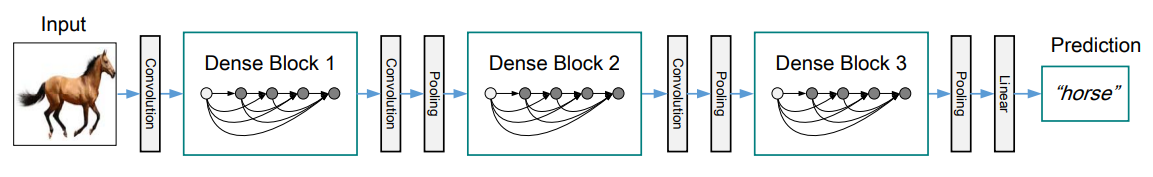
\includegraphics[width=\linewidth]{figures/densenet}
	\caption{\textmd{DenseNet architecture}}
	\label{fig:densenet-model}
\end{figure}


\begin{equation}
\label{eq:ce}
CE(C, C^\prime) =  \frac{|U| - D_{max}}{|U|},
\end{equation}


\begin{table}[ht]
\small
\centering
\begin{threeparttable}
\renewcommand{\arraystretch}{1.3}
\caption{Specifications of the Deep Learning Benchmark Image Datasets}
\label{tab:deep-datasets}
\centering
\begin{tabular}{c|ccc}
\hline
\bfseries  Datasets & \bfseries Resolution & \bfseries Channels & \bfseries Classes\\
\hline
\gls{cifar10} & 32 x 32 & 3 & 10 \\
\gls{svhn} & 32 x 32 & 3 & 10 \\
MNIST & 28 x 28 & 1 & 10 \\
FashionMNIST & 28 x 28 & 1 & 10 \\
\hline
\end{tabular}
\end{threeparttable}
\end{table}


\begin{algorithm}[!ht]
Initialize parameters;

\For{epoch $\gets$ 0 \textit{\textbf{to}} $epoch_{max}$}
{
	Choose a random input pattern $\boldsymbol{x}$;

	\eIf{\text{condition}}
    {
    	Run X;

    } {
    	Run Y.;
    }
}

\caption{Algorithm}
\label{alg:algorithm}
\end{algorithm}



\begin{references}
	\bibliography{default_content/references}
\end{references}

\end{document}
